\pdfoutput=1

\documentclass{article}

\usepackage[preprint]{tmlr}

\usepackage{amsmath,amssymb,amsfonts}
\usepackage{booktabs}
\usepackage{graphicx}
\usepackage{hyperref}
\usepackage{xcolor}
\usepackage{microtype}

\renewcommand{\arraystretch}{1.25}
\emergencystretch=1.5em

\title{Interaction Structure in a Belief-Tracking Circuit}

\author{\name Elliot Tower \\
      \email elliot@elliottower.ai}

\begin{document}
\maketitle

\begin{abstract}
\citet{prakash2025lookback} describe three ``lookback'' sub-mechanisms in Llama-3.1-70B-Instruct as instances of one computation. Their strongest causal design patches two token groups separately and together, and the three measurements plus the unpatched condition form a complete two-player coalition function, so the Walsh--Hadamard interaction coefficient between the groups is exact rather than estimated. We compute it for Qwen2.5-14B-Instruct at 24 layer-by-mechanism cells ($n = 200$ story pairs each). The two sub-mechanisms carry pairwise interactions of opposite sign, each saturated at the extreme the measurement admits. The binding lookback at layers 24--34 is an exact parity function: patching either token group alone transfers the counterfactual answer at IIA $= 1.0$, patching both transfers it at $0.0$, and both order-1 coefficients are exactly zero, placing $100\%$ of the non-constant spectrum at order~2. The answer lookback at layers 32--38 is a conjunction: singles at $0.005$ and $0.000$, pair at $1.0$, $w_2 = +0.249$ against a ceiling of $+0.25$. Sign stability is $1.000$ across $10{,}000$ bootstrap draws in every cell above the additive tolerance. A summary that reports each token group's marginal contribution assigns the binding lookback two zeros and describes nothing that happens in it. We report the decomposition as a follow-up to a pre-registered cross-model experiment, not as a registered prediction.
\end{abstract}

\noindent\textbf{Keywords:} mechanistic interpretability, interaction decomposition, interchange interventions, belief tracking, epistasis


\section{Introduction}

A circuit claim names several components and asserts that they produce a behavior together. Where the claim also carves the circuit into stages, it asserts something further: that the stages are the same kind of thing. \citet{prakash2025lookback} identify three ``lookback mechanisms'' for belief tracking in Llama-3.1-70B-Instruct---binding, answer, and visibility---operating at non-overlapping layer ranges, on different token types, with per-layer subspace ranks that differ by an order of magnitude. The paper treats them as one computation, dereferencing a pointer via attention, and generalizes across models on that basis.

Testing whether two stages are one kind of thing requires a measurement that distinguishes them. Marginal importance does not: two components can carry identical individual effects and combine in opposite ways. The quantity that separates them is the interaction, the deviation of the joint effect from the sum of the singles.

\citet{prakash2025lookback} already collect the data this requires. Their mismatch test patches the recalled tokens alone, the lookback tokens alone, and both, on the reasoning that patching one alone leaves address and pointer inconsistent. With the unpatched condition, these are all four values of a two-player coalition function. The Walsh--Hadamard decomposition of four values is exact---no sparse recovery, no regularization, no held-out set---so the interaction coefficient between the two token groups is determined, not estimated.

We compute that coefficient for Qwen2.5-14B-Instruct across 24 layer-by-mechanism cells. The binding and answer lookbacks carry interactions of opposite sign, each at the boundary of the attainable range. The binding lookback has no additive component at all: its order-1 coefficients are exactly zero over six consecutive layers, and every measurable effect lives in the interaction term.


\section{Coalition Function}

Write $x = (x_0, x_1) \in \{0,1\}^2$, where $x_0 = 1$ patches the recalled tokens and $x_1 = 1$ patches the lookback tokens. Let $v(x)$ be interchange intervention accuracy: the fraction of story pairs on which the model returns the counterfactual answer under the indicated patch.

The empty coalition is zero by construction. Pairs are filtered so that the model returns the clean answer on the clean prompt and the counterfactual answer on the counterfactual prompt, and IIA counts matches against the counterfactual target. With no patch applied the model returns the clean answer, which differs from the counterfactual target by the definition of the pair. So $v(0,0) = 0$ exactly, and the remaining three cells are the three conditions the mismatch test already reports.

The four values admit a unique Walsh--Hadamard decomposition,
\begin{equation}
  v(x) = \sum_{S \subseteq \{0,1\}} w_S\, \chi_S(x),
  \qquad
  \chi_S(x) = (-1)^{\sum_{i \in S} x_i},
  \qquad
  w_S = \tfrac{1}{4} \sum_{x} v(x)\, \chi_S(x),
\end{equation}
following the convention of \citet{poelwijk2016context}. The order-1 coefficients $w_{\{0\}}$ and $w_{\{1\}}$ give each token group's contribution averaged over the state of the other; the order-2 coefficient $w_2 \equiv w_{\{0,1\}}$ gives the deviation from additivity. Positive $w_2$ is super-additive, negative is sub-additive. Following \citet{tower2026epistatic} we also report the masking value $M = -w_2$, on which positive means masking and negative means synergy.

Because $v \in [0,1]$ with $v(0,0)$ pinned at zero, $w_2$ is bounded: it reaches $-0.5$ when both singles transfer perfectly and the pair transfers nothing, and $+0.25$ when neither single transfers and the pair transfers perfectly. Reporting $w_2$ against these bounds gives a saturation fraction, so a coefficient can be read as a proportion of the largest interaction the design can express.

The energy identity $\sum_S w_S^2$ partitions the variance by order. The fraction at order 2 states how much of the circuit's measurable behavior requires both token groups jointly, and its complement states how much an additive summary retains.


\section{Interaction Coefficients}

We apply the decomposition to \citet{prakash2025lookback}'s three-condition mismatch test, run on Qwen2.5-14B-Instruct with $n = 200$ filtered story pairs per condition, 12 layers per lookback type. Clean accuracy is $1.0$ in every cell. Table~\ref{tab:interaction} gives the coefficients at the layers where each mechanism is established; Figure~\ref{fig:coefficient} gives the full layer profile.

\begin{table}[t]
\centering
\caption{Order-2 Walsh coefficients for the two token groups of the mismatch test, Qwen2.5-14B-Instruct, $n = 200$ pairs per cell. Saturation is $w_2$ as a fraction of the bound it approaches ($-0.5$ for masking, $+0.25$ for synergy). Order-2 energy is the fraction of non-constant Walsh energy at order~2. Confidence intervals resample each cell as an independent binomial; the three patched conditions share the same filtered pairs, so the paired interval is narrower than the one reported.}
\label{tab:interaction}
\vspace{0.5\baselineskip}
\begin{tabular}{llccccc}
\toprule
Mechanism & Layers & singles & pair & $w_2$ & saturation & order-2 energy \\
\midrule
Binding & 12--18 & $1.000$ / $0.010$ & $0.965$--$1.000$ & $-0.011$ & $0.02$ & $0.001$ \\
Binding & 20--22 & $1.000$ / $0.343$ & $0.425$--$0.445$ & $-0.227$ & $0.45$ & $0.399$ \\
Binding & 24--34 & $1.000$ / $0.999$ & $0.000$ & $-0.499$ & $1.00$ & $1.000$ \\
\midrule
Answer & 16--28 & $0.005$ / $0.000$ & $0.005$--$0.020$ & $+0.000$ & $0.01$ & $0.000$ \\
Answer & 30 & $0.010$ / $0.000$ & $0.440$ & $+0.108$ & $0.43$ & $0.323$ \\
Answer & 32--38 & $0.020$ / $0.010$ & $1.000$ & $+0.242$ & $0.97$ & $0.320$ \\
\bottomrule
\end{tabular}
\end{table}

\begin{figure}[t]
\centering
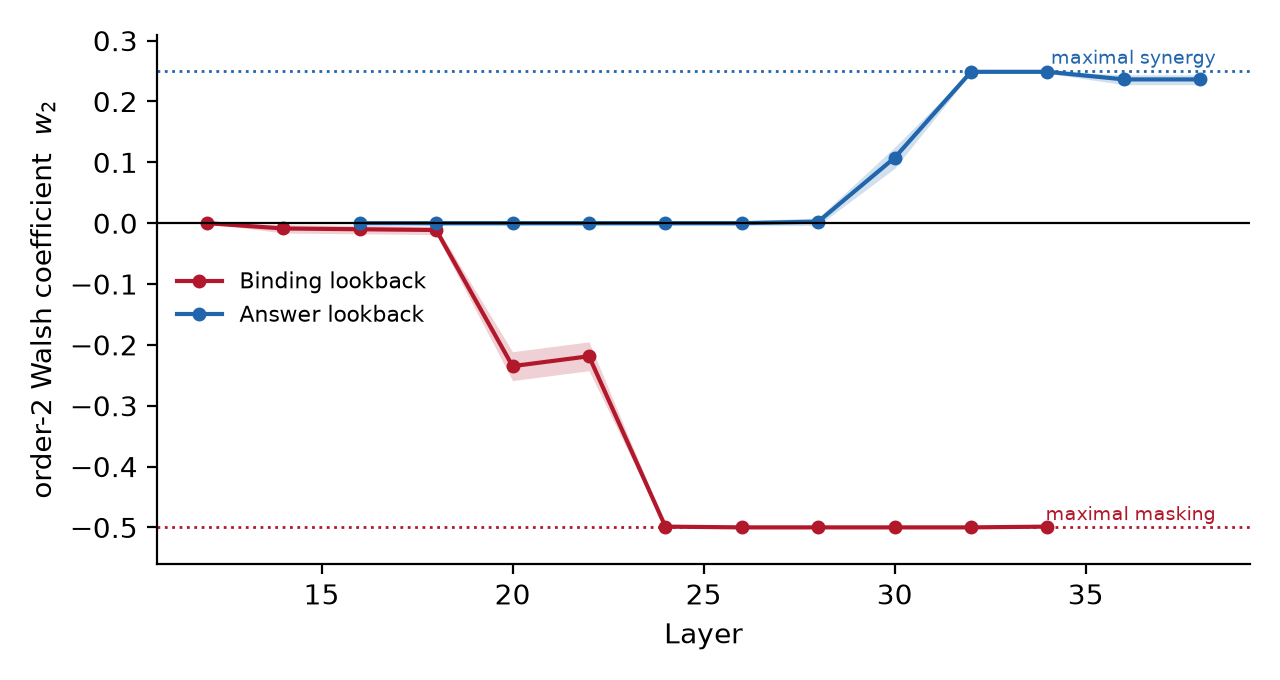
\includegraphics[width=0.72\textwidth]{figures/interaction_coefficient.pdf}
\caption{Order-2 Walsh coefficient by layer for the two lookback mechanisms in Qwen2.5-14B-Instruct. Dotted lines mark the bounds the design admits, $-0.5$ and $+0.25$. The binding lookback reaches the masking bound at layer 24 and holds it through layer 34; the answer lookback reaches $97\%$ of the synergy bound at layer 32 and holds it through layer 38. Shaded bands are 95\% bootstrap intervals over $10{,}000$ draws, treating cells as independent binomials.}
\label{fig:coefficient}
\end{figure}

\paragraph{Binding lookback: parity.}
From layer 24 onward the coalition values are $v = (0, 1, 1, 0)$ to within one pair in 200. Patching the recalled tokens alone transfers the counterfactual answer on every pair. Patching the lookback tokens alone transfers it on every pair. Patching both transfers it on none. Both order-1 coefficients are exactly zero, and $w_2 = -0.499$, the masking bound. The fraction of non-constant energy at order 2 is $1.000$: the function is parity over the two token groups, and it has no additive part.

\paragraph{Answer lookback: conjunction.}
From layer 32 onward the coalition values are $v = (0, 0.005, 0, 1)$. Neither token group transfers the counterfactual answer alone; together they transfer it on every pair. Here $w_2 = +0.249$ against a ceiling of $+0.25$, and the order-2 energy fraction is $0.331$, the value a conjunction takes. This is the signature \citet{prakash2025lookback} predict, and on the answer lookback it holds.

\paragraph{Transitions.}
Neither pattern is present at the earliest layers tested. The binding lookback is nearly additive at layers 12--18, where the recalled tokens alone already transfer the answer and the lookback tokens contribute $0.010$; it passes through a mixed regime at layers 20--22 ($w_2 = -0.235$ and $-0.219$, order-2 energy $0.43$ and $0.37$) before saturating. The answer lookback is flat at zero through layer 28 and passes through layer 30 at $w_2 = +0.108$. The sign of the interaction is therefore a property of a layer range rather than of a mechanism as a whole, and both ranges have an interior boundary where it changes.

Sign stability across $10{,}000$ bootstrap draws is $1.000$ in every cell whose coefficient exceeds the additive tolerance of $0.01$.


\section{Cost of an Additive Summary}

\citet{leemann2024slalom} prove that attention architectures cannot represent additive models over input tokens. Whether additivity also fails between the parts of a circuit is a separate question, and the two mechanisms here answer it differently. The answer lookback retains two thirds of its energy at order 1, so a report of marginal contributions preserves most of what it does. The binding lookback retains none.

For binding at layers 24--34 the marginal contribution of each token group, averaged over the state of the other, is zero. The recalled tokens transfer the answer when the lookback tokens are untouched and block it when they are patched, in exactly compensating amounts. A method that reports per-component importance therefore assigns both groups a score of zero, which is correct as an average and describes nothing that occurs at any layer. The whole of the mechanism's behavior sits in a term such a method does not compute.

The two mechanisms are also distinguished by nothing else the design measures. Both reach IIA $1.0$ under some patch. Both have clean accuracy $1.0$. Read through marginals, the binding lookback at layer 26 and the answer lookback at layer 34 are a pair of components with high causal relevance. Read through the interaction, one is a parity function and the other a conjunction.


\section{Dependency Structure and the Unity Claim}

\citet{prakash2025lookback} test Qwen2.5-14B-Instruct and Llama-3.1-405B-Instruct with full-residual interchange interventions, note that ``subspace interchange intervention experiments were not conducted,'' and conclude that these models ``employ the same underlying mechanism.'' Full-residual patching replaces all information at a position at once, so it cannot separate address from payload and cannot see a dependency between them.

The mismatch signature transfers for the answer lookback and inverts for binding. On the paper's own reading of the test---singles fail because address and pointer disagree, the pair succeeds because they are made consistent---the binding result says the two token groups in Qwen each carry a sufficient copy of the counterfactual state, and patching both installs two copies that cancel. Whatever produces that is not the mechanism the test was designed to detect.

Applying the sign convention from genetics is tempting here and we do not. \citet{benzer1955} decides one unit or two from the phenotype of a double perturbation, with sub-additivity reading as one pathway and super-additivity as two. That convention was defined for loss-of-function perturbations. Interchange interventions install a value rather than remove one, and ``the second hit has nothing left to break'' has no counterpart when both hits write. The coefficients are reported; the same-unit verdict is not.

What the coefficients do support is narrower. Two of the three sub-mechanisms that \citet{prakash2025lookback} group under one name have pairwise interactions of opposite sign in a model the paper claims the mechanism generalizes to, and the difference is maximal rather than marginal. A claim of shared computational type has to survive that, and the paper's evidence---full-residual patching, which is blind to the interaction---cannot address it either way.


\section{Audit Context}

The mismatch test reanalyzed here was run as part of a pre-registered validity audit of \citet{prakash2025lookback} against the 36 criteria of \citet{tower2026mechval}. Fifteen experiments were registered in timestamped amendments before results. Table~\ref{tab:audit} lists those that completed, for context on what the surrounding record contains.

\begin{table}[t]
\centering
\caption{Completed experiments from the pre-registered audit. Predictions marked $\dagger$ were overturned by the data, in each case in the audited claim's favor.}
\label{tab:audit}
\vspace{0.5\baselineskip}
\begin{tabular}{llp{6.4cm}}
\toprule
Experiment & Criterion & Result \\
\midrule
Positive control replication & Replication & Four subspaces replicate within $\pm 0.13$ on a minor model version update; L36 does not ($0.75$ reported, $0.23$ observed) \\
Cross-template transfer & Construct generality & L38 IIA $= 0.957$, L52/L53 $= 0.783$ on a held-out template ($n = 23$) \\
Cross-task transfer & Discriminant validity & L38 reaches $0.529$ on factual recall and $0.886$ on action recall; L52 and L53 reach $0.0$ on both \\
Question-framing control$^\dagger$ & Construct definition & Belief framing IIA $= 1.0$; reality-state framing $0.82$--$0.92$ over the same pairs ($n = 250$) \\
Distractor insertion & Specificity & Viable pairs fall to $21$ under early insertion and $0$ under mid and late insertion \\
True false-belief test$^\dagger$ & Discriminant validity & IIA $= 0.975$ on stories where belief diverges from reality, against a registered prediction of $< 0.30$ \\
Observability dissociation$^\dagger$ & Discriminant validity & IIA $= 0.988$ on observed-other knowledge, against a registered prediction of $< 0.30$ \\
Subspace ablation & Necessity & Zero-ablation costs $0.00$--$0.12$ accuracy; four of six subspaces are removable \\
Rescue reversibility & Reversibility & Ablated $0.92$, rescued $1.0$, wrong-sample rescue $0.545$, random-subspace rescue $0.93$ \\
Cross-model mismatch & Cross-model & The subject of this paper \\
\bottomrule
\end{tabular}
\end{table}

The audit as a whole is reported separately. The decomposition here does not depend on any of its other results: it uses the mismatch measurements alone.


\section{Limitations}

\paragraph{One model, two mechanisms.}
The coefficients are for Qwen2.5-14B-Instruct. The corresponding measurement for Llama-3.1-70B-Instruct would require the same three-condition test on that model; \citet{prakash2025lookback} report their Llama mismatch result as a figure without tabulated values, and their released results file records single-condition IIA per layer only. The cross-model comparison here therefore contrasts our Qwen coefficients against the paper's stated design expectation, not against a matched Llama measurement. The visibility lookback was not tested.

\paragraph{Two players.}
An order-2 energy fraction over two players is not comparable to the same quantity over a fifteen-head circuit, where three non-constant coefficients become $32{,}767$. What carries weight in the binding result is that the order-1 coefficients are exactly zero, not that the fraction reaches one.

\paragraph{No reliability gate.}
\citet{tower2026epistatic} gates interaction coefficients on split-half reliability across prompts, with a Spearman--Brown floor of $0.6$. The mismatch test stores per-condition counts rather than per-pair outcomes, so no split is available. The bootstrap reported here resamples cells as independent binomials, which ignores the shared pair set and overstates the interval width.

\paragraph{Token groups, not components.}
The two players are token positions under patching, not attention heads or subspaces. The interaction is between what those positions carry, and a component-level decomposition of the same mechanism would be a different measurement.

\paragraph{Registration status.}
The cross-model mismatch experiment was pre-registered. This decomposition was derived from its results afterward and is a follow-up, not a registered prediction.


\section*{Data and Code Availability}

The interaction coefficients, the coalition values they are computed from, and the analysis conventions are at \texttt{results/walsh\_interaction/qwen\_mismatch\_walsh.json}. The decomposition script is \texttt{experiments/walsh\_interaction\_qwen.py}; the underlying measurements are at \texttt{results/qwen\_mismatch/}. Pre-registration amendments are git-tagged.

\bibliography{references}
\bibliographystyle{tmlr}

\end{document}
